% Instructions to change to html version:
% Comment out:
%  minipage, multicols,columnbreak, mathbf, hrule
% Replace all: \begin{minipage} \end{minipage} \begin{mulicols}  \begin{mulicols}  \columnbreak  \begin{framed} \end{framed} \hrule
% Search for \mathbf
% Replace \\] with \[ and \) with \(
% Enclose graphics in figure environments and add captions
% Re-tag \df environments as sections, subsections, etc.
% Command Line Code to Create html version:
%First: pdflatex -shell-escape filename.tex                                   
%Second, for each figure: inkscape "filename-figure1.pdf" -o "filename-figure1.png"
% Third: htlatex filename.tex "ht5mjlatex.cfg, charset=utf-8" " -cunihtf -utf8"

\documentclass[10pt]{article}

%\usepackage{tikz, pgf,pgfplots,wasysym,array}
%\usepackage{wasysym,array}

\usepackage{amsmath,amssymb}

\ifdefined\HCode
  \def\pgfsysdriver{pgfsys-tex4ht-updated.def}
\fi 
%\ifdefined\HCode
%  \def\pgfsysdriver{pgfsys-dvisvgm4ht.def}
%\fi 
\usepackage{tikz}
\usetikzlibrary{calc,decorations.markings,arrows}
\usepackage{pgfplots}

\pgfplotsset{compat=1.12}
\usepackage{myexternalize}
\usetikzlibrary{calc,decorations.markings,arrows}
\usepackage{framed}
\usepackage[none]{hyphenat}

\input{../../../common/1336_header_test.tex}
% % !tex root = ./exam_2.tex
\usepackage[nomessages]{fp}% 
\usepackage{rotating}
\usepackage{graphicx}
\usepackage{sectsty}
\usepackage{xparse}
\usepackage{tikz}
\usepackage{pgf,pgfplots}
	% For the histogram ?
	\pgfdeclarelayer{background}% determine background layer
	\pgfsetlayers{main,background}% order of layers

\usepackage{tkz-berge}
\usetikzlibrary{calc,graphs,arrows,backgrounds,decorations.pathreplacing}
%Not found:\usetikzlibrary{graphs.standard,quotes}
\usetikzlibrary{shapes}
		\tikzset{
		  dot hidden/.style={},
		  line hidden/.style={},
		  dot colour/.style={dot hidden/.append style={color=#1}},
		  dot colour/.default=black,
		  line colour/.style={line hidden/.append style={color=#1}},
		  line colour/.default=black
		}
\NewDocumentCommand{\rot}{O{45} O{1em} m}{\makebox[#2][l]{\rotatebox{#1}{#3}}}%


\begin{document}



\newcommand{\an}{\lbrace a_n \rbrace}
\newcommand{\Sum}{\sum_{n=1}^\infty }
\newcommand{\Sumzero}{\sum_{n=0}^\infty }

\everymath{\displaystyle}

\renewcommand{\myTitle}{	MATH 1336: Calculus III}

\renewcommand{\mySubTitle}{Section 8.7, Part 1: Intro to Taylor \& Maclaurin Series}% \vspace*{-.25in}}
%~\hfill Name: \underline{~~~~~~~~~~~~~~~~~~~~~~~~~~~~~~~~~~~~~~~~~~~~~~~}

%\lectTitle{\vspace*{-.5in}\myTitle}{\vspace*{.1in}\mySubTitle \vspace*{-.2in}}

\title{\mySubTitle}\date{}
\maketitle


\hspace*{-.8in}%\begin{minipage}{1.25\textwidth}

\setlength{\columnseprule}{.4pt}
\setlength{\columnsep}{3em}

%\begin{framed}
\section*{Taylor \& Maclaurin Series Key Idea:}

%\begin{minipage}{.6\textwidth}
%\hspace*{-.15in}
\begin{figure}[!h]
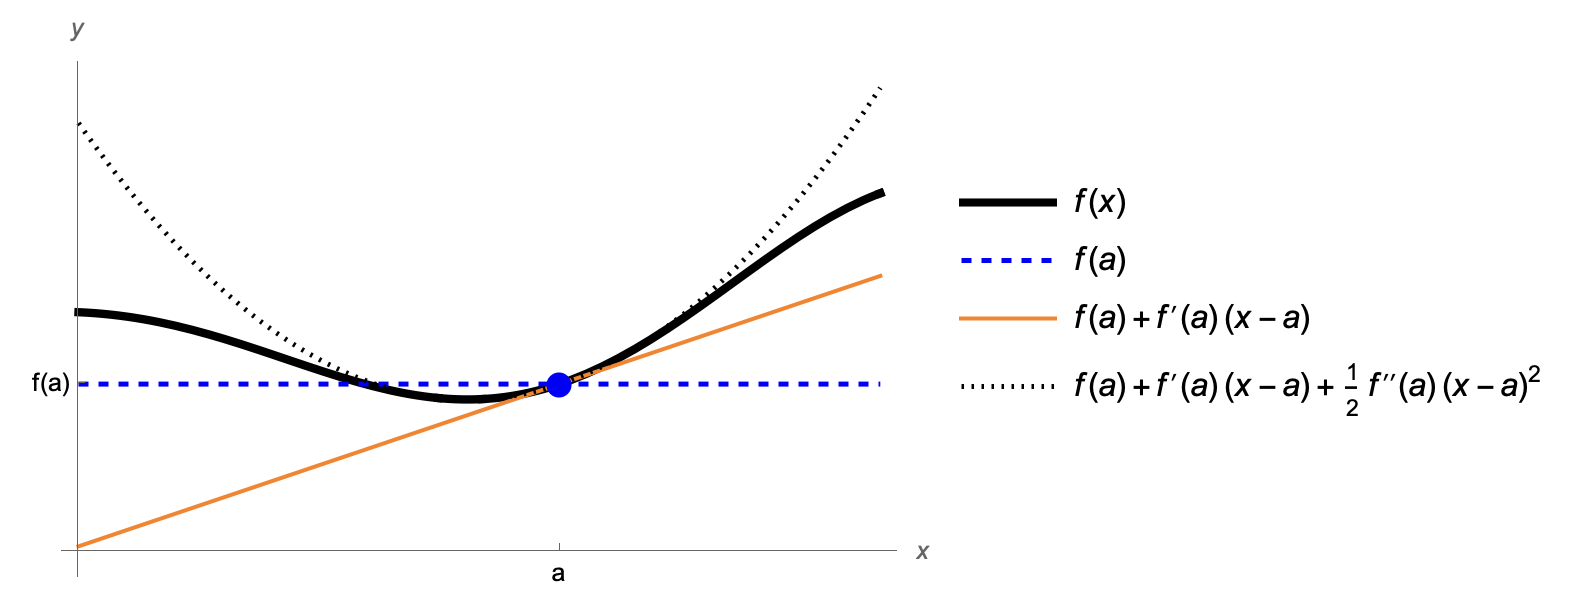
\includegraphics[width=1.05\textwidth]{Ch8s7-Taylor2.png}
%\caption{Graph showing a function \(f(x)\) and the constant approximation: \(f(a)\), the linear approximation: \(f(a) + f'(a)(x-a)\), and the quadratic approximation:  \(f(a) + f'(a)(x-a)+\frac{1}{2}f''(a)(x-a)^2\).}
\end{figure}
%\end{minipage}
%\hspace*{.1in}
%\begin{minipage}{.35\textwidth}
To build a polynomial of degree \(n\) that approximates the function \(f(x)\) well near \(x=a\), make sure that it matches the first \(n\) derivatives of \(f\) \textit{exactly} at \(x=a\).\\~\\
 The more derivatives we match, the better our approximation should be!\\~\\

%\textbf{Notation:}
%\begin{itemize}
%%\item \textbf{Note:} We are ``allowed'' to represent \(f\) as the series above when \(x\) is within the radius of convergence, \(R\), i.e.: \(|x-a|<R\).
%\item \(f^{(n)}(x)\) is the n\(^{th}\) derivative of \(f\) w.r.t. \(x\)%with respect to \(x\)
%\item \(f^{(0)}(x) = f(x)\)
%\item \(0! = 1\)
%%\item \textbf{Taylor Polynomial -vs- Taylor Series:} A Taylor Polynomial of degree \(n\) (or order \(n\)) \(T_n(x)\) terminates after the \((x-a)^n\) term, while a Taylor Series typically has infinitely many terms.
%%\(
%%T_n(x) = f(a) + f^{(1)}(a)(x-a) + \frac{f^{(2)}(a)}{2!}(x-a)^2+\ldots+\frac{f^{(n)}(a)}{n!}(x-a)^n\\
%%\)
%\end{itemize}
%\end{minipage}

%\hrule
\vspace*{.1in}

\section*{Taylor Polynomials -vs- Taylor Series:}
 A Taylor Polynomial of degree \(n\) (or order \(n\)) \(T_n(x)\) terminates after the \((x-a)^n\) term:
\(
T_n(x) = f(a) + f^{(1)}(a)(x-a) + \frac{f^{(2)}(a)}{2!}(x-a)^2+\ldots+\frac{f^{(n)}(a)}{n!}(x-a)^n,\\
\)
while a Taylor Series is a power series centered at \(x=a\) that typically has infinitely many terms. A Taylor Series that is centered at \(x=0\) is given a special name: Maclaurin Series.\\~\\

%\hrule
\vspace*{.1in}

\section*{Taylor Series}% for \(f(x)\) centered at \(a\):}
%\vspace*{-.1in}
%\begin{eqnarray*}
\[
f(x) = \sum_{n=0}^\infty \frac{f^{(n)}(a)}{n!}(x-a)^n = f(a) + f^{(1)}(a)(x-a) + \frac{f^{(2)}(a)}{2!}(x-a)^2
\]
\[
 +\ \frac{f^{(3)}(a)}{3!}(x-a)^3+\frac{f^{(4)}(a)}{4!}(x-a)^4+\ldots
\]
%\end{eqnarray*}

%\vspace*{.1in}
%
%
\section*{Maclaurin Series}% for \(f(x)\):}
\vspace*{-.1in}
%\begin{eqnarray*}
\[
f(x) = \sum_{n=0}^\infty \frac{f^{(n)}(0)}{n!}x^n = f(0) + f^{(1)}(0)x 
+ \frac{f^{(2)}(0)}{2!}x^2 + \frac{f^{(3)}(0)}{3!}x^3+\frac{f^{(4)}(0)}{4!}x^4+\ldots
\]
%\end{eqnarray*}
%% \columnbreak
 
%\hrule
\vspace*{.1in}

\section*{ Notation \& Other Details:}
\begin{itemize}
\item \textbf{Note:} We are ``allowed'' to represent \(f\) as the series above when \(x\) is within the radius of convergence, \(R\), i.e.: \(|x-a|<R\).
\item \(f^{(n)}(x)\) is the n\(^{th}\) derivative of \(f\) with respect to \(x\)
\item \(f^{(0)}(x) = f(x)\)
\item \(0! = 1\)
%\item \textbf{Taylor Polynomial -vs- Taylor Series:} A Taylor Polynomial of degree \(n\) (or order \(n\)) \(T_n(x)\) terminates after the \((x-a)^n\) term, while a Taylor Series typically has infinitely many terms.
%\(
%T_n(x) = f(a) + f^{(1)}(a)(x-a) + \frac{f^{(2)}(a)}{2!}(x-a)^2+\ldots+\frac{f^{(n)}(a)}{n!}(x-a)^n\\
%\)
\end{itemize}
%  \vspace*{.25in}
%  
%  %\hrule
%  \vspace*{.1in}
  
  %\end{framed}
  %\end{minipage}
  
  %\begin{framed}

\section*{Strategy for Finding Taylor/Maclaurin Series:}
\begin{enumerate}[(1)]
\item Evaluate the first 4 or 5 derivatives of \(f(x)\) at \(x=a\).
\item Look for a pattern that describes the coefficient of the \((x-a)^n\) term:
\(\frac{f^{(n)}(a)}{n!}\).
\item If the ``pattern'' includes alternating signs, use either \((-1)^n\) or \((-1)^{n-1}\), depending on whether the first term is positive or negative.
\end{enumerate}


%\end{multicols}

%\end{framed}

%%\end{minipage}

\vfill

\section*{Examples we will work through together:}

\begin{enumerate}[{Example }1:]
%\addtocounter{enumi}{4}


\item Find the Maclaurin Series for \(f(x) = e^x\). \vfill
\item Find the radius of convergence of the Maclaurin Series for \(f(x) = e^x\). \vfill
\item Find the Taylor Series for \(f(x) = e^x\) centered at \(x=10\).\vfill


\end{enumerate}

%\pagebreak

\section*{Problems for Group Work}

\begin{enumerate}[{Problem }1:]
\item Find the Maclaurin Series for \(f(x) = \sin(x)\).\vfill \label{sin}
\item Use your answer to Problem \ref{sin} to discover the Maclaurin Series for \(\cos(x)\).\vfill
\item Find the third order Taylor Polynomial, \(T_3(x)\) for \(f(x) = \ln(x^2)\), centered at \(a=1\).\vfill


\end{enumerate}
\end{document}
